\chapter{Supersymmetry}
\label{sec:sup}
\section{Introduction}
\label{sec:introduction}%%%kazakov 2006, theory and phenomenology of sparticles, guía d e la teoría cuántica de campos 
Supersymmetry (henceforth SUSY) is a framework that constitutes one of the main alternatives for BSM Physics. Postulated in the \red{70s} as a graded Lie algebra (with conmutators and anticonmutators), allowed by the Coleman-Mandula theorem ~\cite{ColemanMandula}, possess a unique mathematical nature that allows for the solution of several of the SM caveats that were discussed in the chapter before. It is being searched for in several experiments, and not yet discovered. Lower limits are set in the scale of SUSY breaking, the so-called scale of new physics. \red{current bounds?}  

SUSY can be seen as a generalization of space-time symmetries in QFT, establishing an invariance under the transformations of fermions to bosons, requiring their number to be the same in nature. Hence, for each boson (fermion) there is a superpartner of fermionic (bosonic) nature. If SUSY wasn't broken, the symmetry would be exact and the masses of the particles would coincide with those of their respective superpartners, which is not observed in nature. Moreover, none of the particles known to date fulfills the quality to be a superpartner, which leads to the conclusion that for Supersymmetry to exist there must be more particles than those seen so far (the double, in the simplest supersymmetric extension of the SM). 

A new quantity number can be introduced within SUSY, R-parity, defined as:
\begin{equation}
R = (-1)^{3B + L + 2S}
\end{equation}
Where B is the baryon number, L the lepton number (both quantities conerved in the SM) and S the spin. Particles with R = 1 are SM particles, while their superpartners have R = -1. Models where R-Parity is conserved (hence, B-L invariance) predict the production of superparticle in pairs, and at least one stable supersymmetric particle, the Lightest Supersymmetric Particle (LSP), thus providing a good candidatefor dark matter. There are also SUSY models where R-parity is violated, allowing the LSP to decay to SM particles. An example of a RPVmodel is the bilinear RPV CMSSM~\cite{RPVCMSSM}.%%% https://indico.cern.ch/event/389531/contributions/929493/attachments/1147997/1646586/RPV-status.pdf,

\section{Points addressed by SUSY}
\label{sec:SUSYpoints}
As mentioned earlier, the success of SUSY lies in the coverage of SM most important \red{pitfalls}. A summary of this is discussed in this section. 
\begin{itemize}
\item \textbf{Unification of forces}: as explained in the \ref{sec:introduction}, gravity is not included in the SM. Nevertheless, given that SUSY algebra is a generalization of Poincaré algebra, it is therefore invariant under general coordinate transformation if it is local. With this, a theory including gravity ({\textit{supergravity}}) can be obtained from SUSY. 
\item \textbf{Gauge hierarchy problem}: Supersymmetry (and supersymmetric partners) lead to the cancellation of quadratic mass terms causing divergences up to the SUSY breaking scale, $M_{SUSY}$, given the relation 
\begin{equation}
\sum_{bosons} m^2 - \sum_{fermions} m^2 = M_{SUSY}^2
\end{equation}
\red{The origin of EWSB can also be explained from radiative electroweak symmetry breaking within SUSY, also explaining the difference between the scales ($M_{SUSY}$ and the Higgs mass).}
\item \textbf{Unification of forces}: as mentioned earlier, the behavior of the coupling constants at high energies hints a \textit{great unification} of forces. This match, while not perfect in the SM, is obtained in a supersymmetric scenario, as it can be seen in figure~\ref{fig:constants}, thanks to the change in the parameters of the renormalization group equations. 
\item \textbf{Matter-antimatter imbalance}: leptogenesis (a scenario in which there is an asymmetry between leptons and antileptons in the early universe) can happen in RPV models, being able to accomnodate the total matter-antimatter imbalance. %%% \red{seesaw mechanism?}%%hypothetical massive bosons leptogenesis? %% https://arxiv.org/pdf/1206.3168.pdf, https://arxiv.org/pdf/0802.2962.pdf
\item \textbf{Dark matter and dark energy}: as pointed out in~\ref{subsec:DarkMatter_DarkEnergy}, most of the origin of dark matter and dark energy remains unexplained in the SM. Supersymmetry can provide several candidates for this, provided R-parity is conserved. More details on the possibilities are discussed in \red{ref}.
\end{itemize}

\section{Supersymmetry breaking} %% theory and phenomenology of susy particles
\label{sec:SUSYbreak}
Supersymmetry breaking is inferred from experimental observation. Without it, the abundance and mass of partners and superpartners would be equal,as said in \ref{sec:introduction}. Moreover, experimental constraints can help reducing the arbitrariness of the MSSM parameters. 

All global continuous symmetries can be broken with an \textit{extra} component of the Lagrangian that breaks the symmetry of the larger part (Heisenberg-Wigner mode), with spontaneous symmetry breaking and the resulting appearance of Goldstone particles, or with a combination of these two methods. The Minimal Supersymmetric Standard Model is an example of the former, and will be discussed in more detail in the following section. 

\section{Minimal Supersymmetrical Standard Model (MSSM)}
\label{sec:MSSM}
The Minimal Supersymmetrical Standard Model is the simplest supersymmetric extension of the SM, containing some general features that do not depend on the choice of model. Among said features is the fact that for each SM partner there is a \textit{superpartner} (\textit{gauginos} for bosons and \textit{sfermions} for fermions), with spin differing 1/2. The particle content is summarized in \ref{tab:parMSSM}.

\begin{table}[h]
  \begin{center}
     \caption{Particle content of the MSSM}
  \label{tab:parMSSM}
  \begin{tabular}{|c|c|c|}
  \hline
  SM & MSSM & Spin \\
    \hline
    gluon ($g$) & gluino $\tilde{g}$ & 1/2\\
    Hypercharge \& Weak bosons & $\tilde{W}^0,\tilde{W}^{\pm}, \tilde{B}^0$ & 1/2 \\
    leptons ($(\nu, l)_L$, $e_R$) & sleptons ($(\tilde{\nu},\tilde{l})_L$, $\tilde{e}_R$) & 0\\
    quarks ($q$) & squarks ($\tilde{q}$) & 0\\
    Higgs field & Higgsinos ($\tilde{H}_u^{\pm}$, $\tilde{H}_d^{\pm}$, $\tilde{H}_u^{0}$, $\tilde{H}_d^{0}$) & 1/2\\
    \hline
  \end{tabular}
  \end{center}
\end{table}

Notice that in the MSSM, as in any supersymmetric scenario, it is required the presence of 2 Higgs bosons in the SM with hypercharge -1 and 1, \red{compatible with FCNC constraints}, as it fulfills the Glashow-Weinberg/Paschos condition(~\cite{Pascos1}, ~\cite{Pascos2}).  Gauginos have spin zero in order to be matter scalars and not gauge bosons. As for the sfermions, the only consistent interacting field theory of spin 3/2 has to include gravity\red{~\cite{Freedman:1976xh}}, hence they have spin 1/2. This theory, known as \textit{supergravity}, includes the superpartner of the \textit{graviton}, known as \textit{gravitino}. It is also worth mentioning that the MSSM, like the SM, fails to explain the number of fermion families. 

The MSSM has some interesing features, such as the improvement in the unification of gauge coupling constants at some high energy scale, $\Lambda$ ,still undetermined but known to be  in the order of $2\times10^{16}$ GeV. This unification is kept if SUSY isbroken at a scale $M_S \leq \mathcal{O} (1 \rm TeV)$. Even if gravity is included, its coupling constant seems to roughly point to the same value at the same $\Lambda$.

%%%% the goal of the BSM search is to find evidence for effects that are present in the theory with a finite value of Lambda, but disappear in the limit Lambda goes to infinity. Limits on electron and neutron EDM require the scale to be larger than 10^7 GeV, while the KK bar mass difference sets a lower bound of about 10^6 GeV on the scale of DS = 2 flavour transitions 

The soft-explicit breaking of the MSSM (or the electroweak symmetry breaking itself) allows for mixing between different sparticles with the same charge and color to happen. This leads to the existence of \textit{charginos} ($\tilde{\chi}^{\pm}_{1,2}$) and \textit{neutralinos} ($\tilde{\chi}^{0}_{1,2,3,4}$), as a combination of gauginos and higgsinos for the former and neutral gauginos for the latter. Sfermion mixing can also happen. \textcolor{blue}{The mixing patterns and mass values of sparticle mass eigenstates depend crucially on the manner of supersymmetry breaking.} 

\subsection{Dark Matter in the MSSM}
%% Introduction
As said before, within the SUSY framework there are several candidates to constitute DM. A common feature they share is their stability. These candidates are:
\begin{itemize}
\item Sneutrino: ruled out in the MSSM because of the current limits on the interaction cross section of dark matter particles with ordinary matter as measured by direct detection experiments
\item Lightest neutralino: the LSP for models conserving R-parity. Depending on its composition it can be of different natures. Said composition comes determined by a unitary 4x4 matrix that diagonalize the neutralino mass matrix, $N$, as seen in \ref{eq:Nneutralino}. \ref{eq:neu1composition}. 
\begin{enumerate}
\item Bino-like: when the term $N_{11}$ dominates the neutralino diagonalization matrix, $N$, fulfilled for $M_1 < \mu$
\item Higgsino-like: when the off-diagonal elements in the mixing matrix ($N_{13}^2 + N_{14}^2$) dominate, for $\mu < M1$ 
\item Wino-like: when the term $N_{12}$ dominates the neutralino diagonalization matrix, $N$, fulfilled for $\mu, M_{1,3} < M_2$
\item Mixed states of the above 
\end{enumerate}
\item Gravitino
\end{itemize}

%%% neutralino mass matrix
\begin{equation}
\left( \begin{matrix}
N_{11} & N_{12} & N_{13} & N_{14} \\ 
N_{21} & N_{22} & N_{23} & N_{24} \\
N_{31} & N_{32} & N_{33} & N_{34} \\ 
N_{41} & N_{42} & N_{43} & N_{44} \\
\end{matrix}\right)
\label{eq:Nneutralino}
\end{equation}

\begin{equation}
\chi_1^0 = N_{11}\tilde{B} + N_{12}\tilde{W} + N_{13} \tilde{H}_d^0 + N_{14}\tilde{H}_u^0
\label{eq:neu1composition}
\end{equation}
%%https://arxiv.org/pdf/1804.05238.pdf

\subsection{MSSM Lagrangian}
\label{sec:MSSMLag}
The MSSM lagrangiang consists of two parts:

\begin{equation}
\mathcal{L}_{\rm MSSM} = \mathcal{L}_{\rm SUSY} + \mathcal{L}_{\rm SOFT}
\end{equation}

Where the first part is just a generalization of the SM lagrangian, and the second part contains the supersymmetry breaking mechanism. 
The corresponding \textit{superpotential} used in $\mathcal{L}_{rm SUSY}$ is of the form:

\begin{equation}
W = \epsilon_{ij}(y_{ab}^{U}Q_a^jU_b^cH_2^i + y_{ab}^{D}Q_a^j D_b^c H_1^i + y_{ab}^{L} L_a^j E_b^c H_1^i + \mu H_1^i H_2^j)
\label{eq:superpotential}
\end{equation}

Where $Q$, $U$ and $D$ represent the squark superfields, $L$ and $E$ the \red{slepton} ones, $y^{U,D,L}$ are the Yukawa couplings and $H_{1,2}$ the Higgs superfields. The only qualitative difference with respect to $\mathcal{L}_{\rm SM}$ is the last term, that accounts for the Higgs mixing. Additional lepton violating leptonic or baryonic number can be added to this superpotential in RPV models. 

Because of gauge invariance, supersymmetry breaking in the MSSM cannot \red{happen spontaneously}. Thus, an explicit term accounting for this breaking appears in the lagrangian, $\mathcal{L}_{\rm SOFT}$, where \textit{soft} refers to the dimension 2 and 3 of the operators.  This breaking is the responsible for the SM particles not to be degenerate with their respective superpartners, as mentioned earlier, having these larger masses. \red{Nonetheless this SUSY breaking, some properties from it remain.} 

%%% singlets?
A possible alternative to the soft-explicit supersymmetry breaking explained before consists in spontaneous symmetry breaking for a given scale, $\Lambda_s$, with a sector of fields that belong to a \textit{hidden} sector and communicates with the \textit{observable} sector with the exchange of fields known as \textit{messengers}, as represented schematically in \ref{fig:hiddensector}. This type of supersymmetry has been extensively searched for in several experiments, with negative results so far \red{REFERENCES}.

\begin{figure} [htb!]
\begin{center}
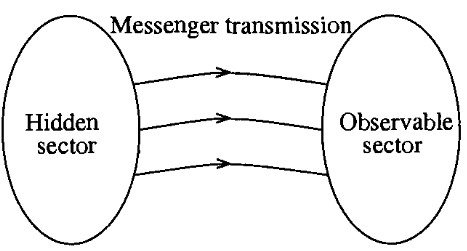
\includegraphics[scale=0.5]{figs/hidden_sector.png}
\caption{Schematic view of the hidden sector \label{fig:hiddensector}}
\end{center}
\end{figure}

The MSSM has 124 free parameters, namely:

\begin{itemize}
\item 18 SM parameters
\item 1 Higgs sector parameter, analogue to the SM Higgs mass
\item 5 real and 3 CP violating phases in the gaugino/higgsino sector
\item 21 squark and slepton masses
\item 36 real mixing angles for squark and slepton mass eigenstates
\item real mixing angles for squark and slepton mass eigenstates
\end{itemize}

The complex phases are usually considered small. Some experiments are capable of measuring some of these parameters individually. Nevertheless, in general this large amount of degrees of freedom \red{spoil the predictive power of the model}. In order to reduce it, \textit{mass universality} is imposed to some particular cases that will be further discussed in the next section. This implies that all spin 0 (1/2) sparticle masses are equal to a universal value $m_0$ ($m_{1/2}$). Another way of reducing the number of parameters is specifying the mechanism that breaks the symmetry, either with gauge fields (Gauge Mediated Supersymmetry Breaking, GMSB)[40] or as a consequence of a dominating super-Weyl anomaly (Anomaly Mediated Supersymmetry Breaking, AMSB). Some of this models will be explained in more detail later. 

%%% Revisar notas --30min

%%% TOTAL: 2h, 2h por la tarde, 2h mañana 


%-- Reduce arbitrariness in the choice of the MSSM parameters  => impose constraints 
%	-- gauge coupling constant unification 
%	-- mZ from EWSB 
%	-- Yukawa copling constant unification 
%	-- Precision measurement of decay rates
%	-- Anomalous magnetic moment of the muon 
%	-- Lower limits on SUSY masses
%	-- DM constraint 
\subsection{CMSSM}
\label{sec:CMSSM}
%% http://www.hep.ph.ic.ac.uk/~tapper/lecture/susy-lecture-1.pdf
%% https://indico.cern.ch/event/136806/contributions/143942/attachments/112092/159367/Wells.pdf
%% http://www.desy.de/~reuter/downloads/marialaach_susy07.pdf
The \textit{constrained} MSSM (hereafter CMSSM) is one of the most popular subversions of the MSSM. In this model, the concept introduced earlier of mass universality is imposed, meaning that for a given GUT scale $\Lambda \sim 2\times 10^{16} \rm GeV$:
\begin{itemize}
\item All scalar masses are set to $m_0$
\begin{equation}
M_{\tilde{l}}^2(\Lambda) = M_{\tilde{q}}^2(\Lambda) \equiv m_0^2 I_3
\end{equation}
\begin{equation}
M_{\tilde{u}}^2(\Lambda) = M_{\tilde{e}}^2(\Lambda) = M_{\tilde{d}}^2(\Lambda) \equiv m_0^2 I_3
\end{equation}
\begin{equation}
m_{H_u}^2 = m_{H_d}^2 = m_0^2
\end{equation}
Where $I_3$ represents the 3x3 identity matrix
\item All gaugino masses are set to $m_{1/2}$
\begin{equation}
m_{\tilde{B}}(\Lambda) = m_{\tilde{W}}(\Lambda) = m_{\tilde{g}}(\Lambda) \equiv m_{1/2}
\end{equation}
\item The trilinear couplings are set to $A_0$
\begin{equation}
A_{\tilde{u}}(\Lambda) = A_{\tilde{e}}(\Lambda) = A_{\tilde{d}}(\Lambda) \equiv A_0 I_3
\end{equation}
\end{itemize} 
These requirements lead to the following relation between the gaugino masses at the TeV scale: 
%\begin{equation} 
%M_{\tilde{g}} : M_{\rm char} : M_{\rm neu} \sim 6 : 4 : 1
%\end{equation}
\begin{equation}
M_1 = \frac{\alpha_s}{\alpha} \sin{\theta_W}^2 M_2 = \frac{3}{5}\cos{\theta_W}^2 M_1
\end{equation}
Which translates into the ratios:
\begin{equation}
M_1 : M_2 : M_3 \approx 1 : 2 : 6
\end{equation}

With these conditions, the CMSSM ends up with a set of 5 free parameters: ($m_0$, $m_{1/2}$, $A_0$, $\tan{\beta} = \frac{v_1}{v_2}$, $\rm sign(\mu)$). The last one refers to the sign of the Higgs self-coupling in the superpotential, while $\tan{\beta} = \frac{v_u}{v_d}$ is the ratio of the vevs from the Higgs doublet. Since gaugino masses run in the same way as the gauge couplings, within the CMSSM the LSP is generally the lightest neutralino. The status of CMSSM in light of current experimental constraints will be reviewed in chapter \ref{sec:CMSSM}.  %% .  \red{supersymmetry invariant higgsino mass? (book)}

%%% main uncertainty comes from the unknown soft terms
%% LSP stable, so that relic neutralinos might survive in the Universe since the Big Bang 
A more restrictive version of CMSSM exists, mSUGRA, where supersymmetry breaking is gravity-mediated. Within this model, the gravitino mass is equal to the scalar mass, $m_{3/2} = m_0$, thus adding a new constraint on the parameters. On the contrary, there are models with more relaxed conditions. An example of these is when the universality condition on the Higgs masses is not applied, hence having Non Universal Higgs Masses (NUHM1 and NUHM2~\cite{Ellis:2002wv}). This adds two extra free parameters, $M_A$, the mass of the CP-odd neutral higgs, $A^0$, and $\mu$, the Higgs self-coupling.  %%%relax the universality conditions on the Higgs masses  on the Higgs mass, 

\subsection{AMSB}
\label{sec:AMSB}
%% Definition : marron
%% mAMSB : blue
%%% Characteristics : red
In the Anomaly Mediated SUSY Breaking (AMSB), the supersymmetry breaking occurs mainly via a loop-induced super-Weyl anomaly. In some scenarios, such breaking is assumed to take place in a different \textit{brane} from respect to the \textit{observable} sector, within the context of \textit{Extra Dimensions}. \textcolor{blue}{The anomaly-mediated SUSY breaking parameters are RG-invariant, being the corresponding masses given as functions of the gauge and Yukawa coupling constants. This helps avoiding a SUSY flavor problem.}

To generate the weak scale masses of the sparticles, the gravitino mass, $m_{3/2}$ must be fairly heavy (of the order of tens of TeV). Ths, it's not affected by Big-Bang nucleosynthesis bounds.  
The gaugino masses $M_{1,2,3}$ are suppressed by loop factors relative to this gravitino mass, and the \red{wino-like states are lighter than the bino-like ones}. The following approximate ratios hold:
\begin{equation}
|M_1| : |M_2| : |M_3| \approx 2.8 : 1 : 7.1
\end{equation}

Within this model, the soft supersymmetry breaking terms can be computed from the gravitino mass, and the soft terms are real and both flavor and renormalization group invariant.
Despite its many advantages, AMSB has a strong drawback: renormalization leads to negative squared masses for sleptons. There are several proposals to cope with this, like the \textit{minimal} AMSB (mAMSB), that will be discussed further in \ref{sec:mAMSB}.

\subsubsection{mAMSB}
\label{sec:mAMSB}

In mAMSB, with the purpose of avoiding \textit{tachyonic} sleptons in AMSB models, a constant contribution ($m_0^2$) is added to all squared scalar masses a the grand unified theory (GUT) scale, $\Lambda_{GUT} \sim 2 \time 10^{16} \rm GeV$. This addition can be mostly related to the presence of extra field(s)in the bulk~\cite{Datta:2001er}, and destroys the aforementioned RG invariance, desirable in order to fulfill the \red{Flavour-Changing-Neutrl-Current (FCNC)} constraint. Nevertheless some characteristics are inherited. 


Both the $\mu$ term and the  to match soft bilinear Higgs coupling, $B_{\mu}$ are parameters of this model too. Given that they determine the Higgs potential:
\begin{equation}
G_F = [2\sqrt{2}(v_2^2 + v_1^1)]^{-1} \simeq 1.7 \times 10^{-5} \rm GeV^{-2}
\label{eq:higgspotential}
\end{equation}
The minimization of \ref{eq:higgspotential} leads to the determination of such paramaters as a function of $\tan{\beta}$. Therefore, the mAMSB model has 3 continuous free parameters, ($m_0$, $m_{3/2}$, $\tan{\beta}$). In addition, the sign of the Higgsino mixing parameter, $\mu$,  is also free. The trilinear soft SUSY-breaking mass terms, like the gaugino masses, are determined by anomalies, therefore they are proportional to the gravitino mass.  

This model has some interesting features, such as:
\begin{itemize}
\item The left and right sleptons are nearly degenerate ($m_{\tilde{l}_R} \approx m_{\tilde{l}_L}$), being stau the lightest slepton. As a consequence, the third and second generation \textit{L-R} mixing angles become significantly larger, reaching the maximal limit at large $\tan{\beta}$.
\item The lightest chargino and neutralino are also almost degenerate ($m_{\tilde{\chi}_1^{\pm}} \approx m_{\tilde{\chi}_1^0}$). This induces to a relatively long-lived $\tilde{\chi}_1^{\pm}$, that decays to a soft charged pion. 
\item Sfermion masses increase lineraly with $m_0$, but also depend on the precise value of $m_{3/2}$.
\item The mass hierarchy between sleptons and gauginos depends on the input parameters.
\item The squark masses are typically very heavy, as they grow with $g_3^4m_{3/2}^2$.
\item The stop masses are relatively high, because of the Higgs mass and the relatively low values of the trilinear couplings.
\item The LSP (lightest neutralino) can be wino-, Higgsino-like or mixed-
\end{itemize}

The most up-to-date likelihood analysis of this model in light of current constraints can be found in~\cite{Bagnaschi:2016xfg}. 
A complete spectra at the best-fit points for the two signs of $\mu$ are shown in Fig. \ref{fig:spectrumno} in the wino-LSP case, where branching ratios exceeding 20\% are indicated by dashed lines. As itcan be seen, a relatively heavy spectrum is favoured in the global fit.
\begin{figure}[htb!]
\begin{center}
  \resizebox{7.5cm}{!}{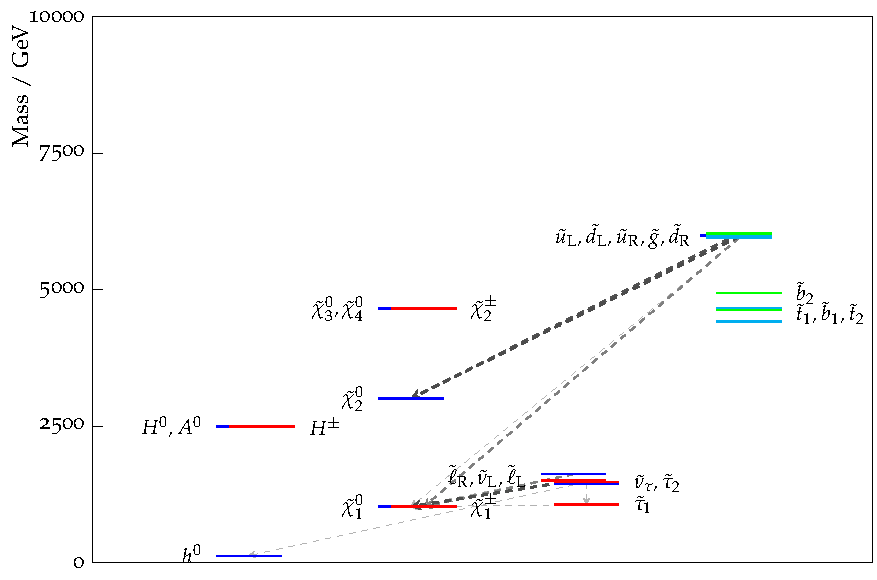
\includegraphics{figs/bfp_posmu_noDM_w_slha.pdf}}\put(-174, +144){\small $\tilde{W}$-LSP  for $\mu>0$, $\Omega_{\tilde{\chi}_1^0}<\Omega_{\rm CDM}$}%above figure
  \resizebox{7.5cm}{!}{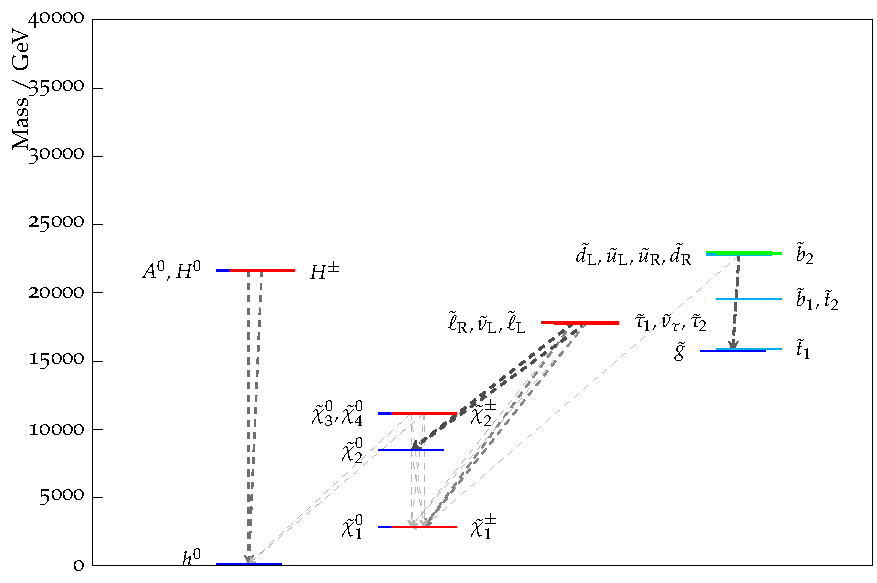
\includegraphics{figs/bfp_negmu_noDM_w_slha.pdf}}\put(-174, +144){\small  $\tilde{W}$-LSP  for $\mu<0$, $\Omega_{\tilde{\chi}_1^0}<\Omega_{\rm CDM}$}%above figure
%\vspace{0.5cm}
%\resizebox{7.5cm}{!}{\includegraphics{bfp_posmu_noDM_h_slha.pdf}}\put(-174, +144){\small  $\tilde{H}$-LSP  for $\mu>0$, $\Omega_{\neu1}<\Omega_{\rm CDM}$}%above figure
%\resizebox{7.5cm}{!}{\includegraphics{bfp_negmu_noDM_h_slha.pdf}}\put(-174, +144){\small  $\tilde{H}$-LSP  for $\mu<0$, $\Omega_{\neu1}<\Omega_{\rm CDM}$}%above figure
\end{center}
\vspace{-0.5cm}
\caption{The spectra of the best-fit points for $\mu > 0$, allowing the LSP to contribute only part of the cold dark matter density. The wino--like LSP (lower) best-fit point is shown, indicating all the decay modes with branching ratios (BRs) above 20\%, with darker shading for larger BRs, and the colours of the horizontal bars reflect particles¿ electric charges.}
%{The range of masses shown for the $\tilde{W}$-LSP $\mu>0$ best fit point (top-left panel) is smaller than the others, since its mass spectrum is considerably lighter.} } }
\label{fig:spectrumno}
\end{figure}

The preferred regions of the $(m_0, m_{3/2})$ planes for $\mu > 0$ (left panel) and $\mu < 0$ (right panel)are shown in  the upper panels of Fig \ref{fig:m0m32UL}~\footnote{{The sharp boundaries at low $m_0$ in the upper panels of Fig \ref{fig:m0m32UL} are due to the stau becoming {the LSP}, and the narrow separation between the near-horizontal portions of the 68 and 95\% CL contours
in the upper right panel of Fig. \ref{fig:m0m32UL} is due to the sharp upper limit on the CDM density.}}. 
It is seen that the wino region allowed at the 95\% CL extends to smaller $m_{3/2}$ for both signs of $\mu$, and also to larger $m_0$ at $m_{3/2} \gtrsim 300 \rm TeV$ when $\mu < 0$. The 68\% CL region extends to much larger $m_0$ and $m_{3/2}$
when $\mu < 0$, and the best-fit point also moves to larger masses than for $\mu > 0$, {though with smaller $\tan{\beta}$}.

\begin{figure}[htb!]
\vspace{0.5cm}
\begin{center}
\resizebox{7.5cm}{!}{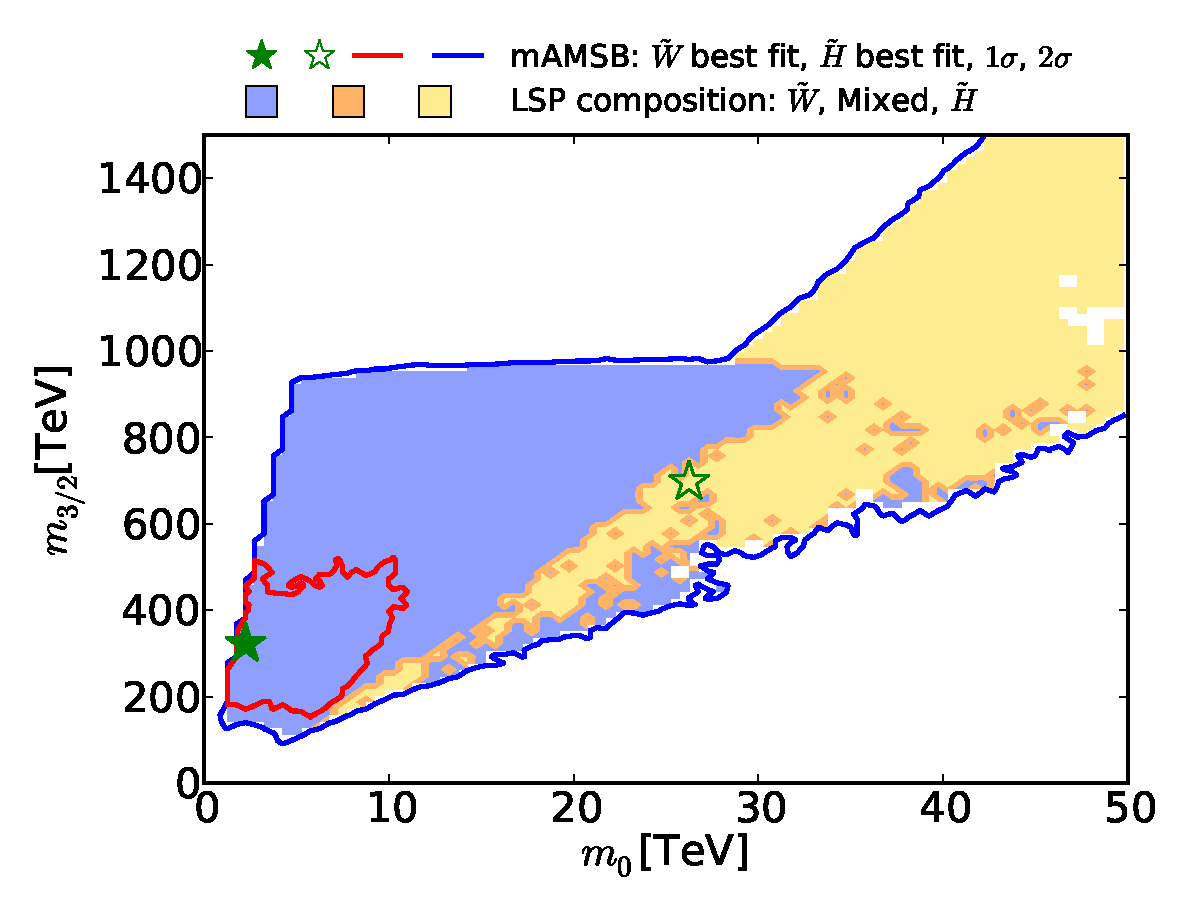
\includegraphics{figs/posmu_noDM_m0TeV50_m32TeV1500_chi2.pdf}}\put(-169, +123){\footnotesize $\mu>0$, $\Omega_{\tilde{\chi}_1^0}<\Omega_{\rm CDM}$}%top left
\resizebox{7.5cm}{!}{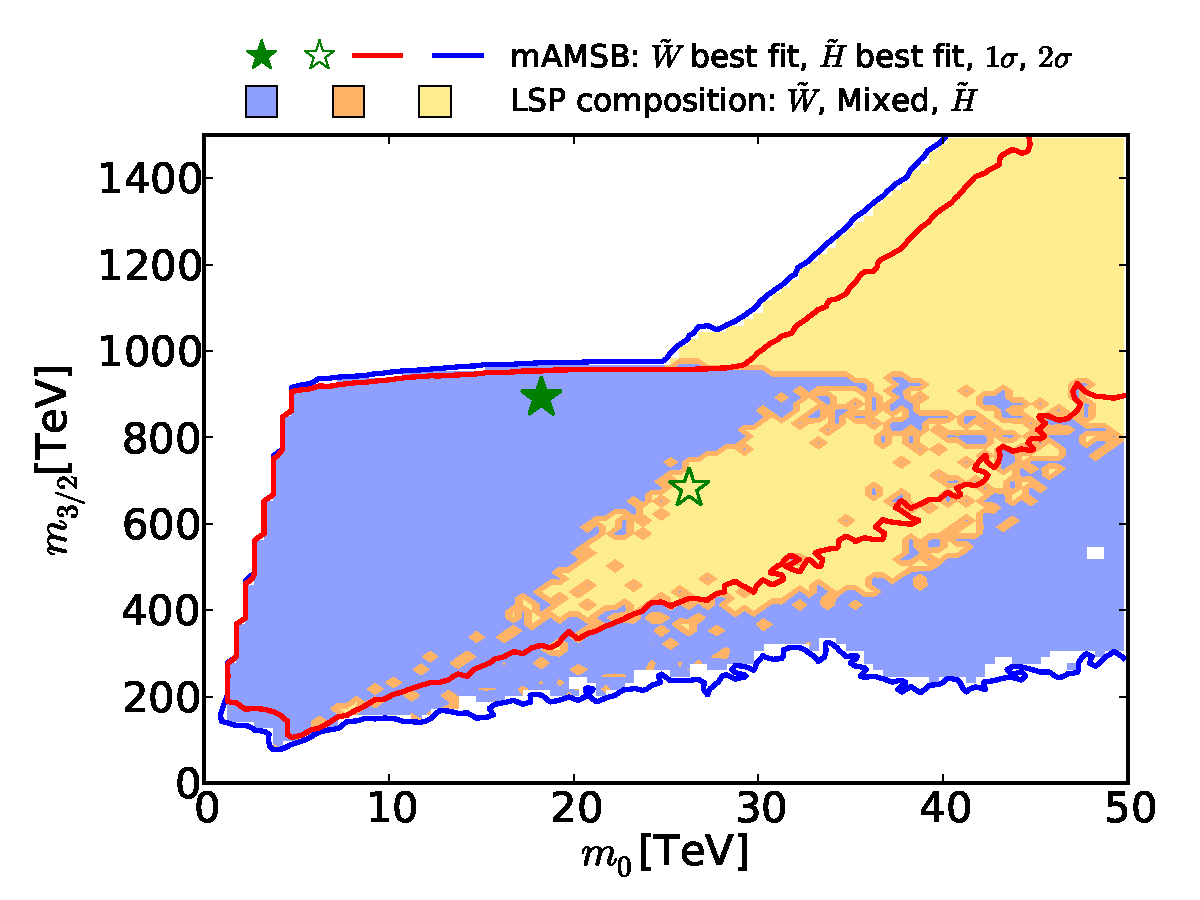
\includegraphics{figs/negmu_noDM_m0TeV50_m32TeV1500_chi2.pdf}}\put(-169, +123){\footnotesize$\mu<0$, $\Omega_{\tilde{\chi}_1^0}<\Omega_{\rm CDM}$}%top left
%\vspace{-3mm}
%\resizebox{7.5cm}{!}{\includegraphics{posmu_noDM_tanb_m32TeV1500_chi2.pdf}}\put(-95, +123){\footnotesize$\mu>0$, $\Omega_{\neu1}<\Omega_{\rm CDM}$}%top right
%\resizebox{7.5cm}{!}{\includegraphics{negmu_noDM_tanb_m32TeV1500_chi2.pdf}}\put(-95, +123){\footnotesize$\mu<0$, $\Omega_{\neu1}<\Omega_{\rm CDM}$}%top right
\end{center}
\vspace{-1.0cm}
\caption{The $(m_0, m_{3/2})$ planes for $\mu > 0$ (left panel) and for $\mu < 0$ (right panel), allowing the $\tilde{\chi}_1^0$ to contribute only part of the CDM density. The best-fit points for the two signs of $\mu$ are indicated by green stars, closed in the
wino-like region and open in the Higgsino-like region.}
%{The shadings are the same as in Fig.~\protect\ref{fig:m0m32}.}}}
\label{fig:m0m32UL}
\end{figure}

Fig \ref{fig:DMdirect_ul} displays the cross section for spin-independent scattering on a proton, $\sigma_p^{\rm SI})$ , versus the neutralino mass, for the case in which the LSP is allowed to contribute only a fraction of the CDM density. As previously, the left plane is for $\mu > 0$, the right plane is for $\mu < 0$, the 1 and 2\,$\sigma$ CL contours are shown as red and blue lines,
and the wino- and Higgsino-LSP regions are shaded in pale blue and yellow. The pale-green-shaded  region represents the range of $\sigma_p^{\rm SI})$\ excluded at the 95\% CL by {a} combination of the latest PandaX and LUX results~\cite{pandax,lux16}, while the purple and {blue} line{s} show the prospective sensitivities of the LUX-Zeplin (LZ), XENON1T {and XENONnT} experiment{s}~\cite{LZ,XENON1T}. Also shown, as a dashed orange line, is the neutrino `floor', below which astrophysical neutrino 
backgrounds would dominate any DM signal~\cite{Snowmass} {(grey region)}. The plot shows good prospects for future DM direct detection experiments when $\mu > 0$, with only a small fraction of the parameter space lying below the neutrino `floor'. {However, when $\mu < 0$ $\sigma_p^{\rm SI})$\ may fall considerably below the `floor', because of cancellations~\cite{cancellations} in the scattering matrix element.}

\begin{figure}[htb!]
\vspace{0.5cm}
\begin{center}
\resizebox{7.5cm}{!}{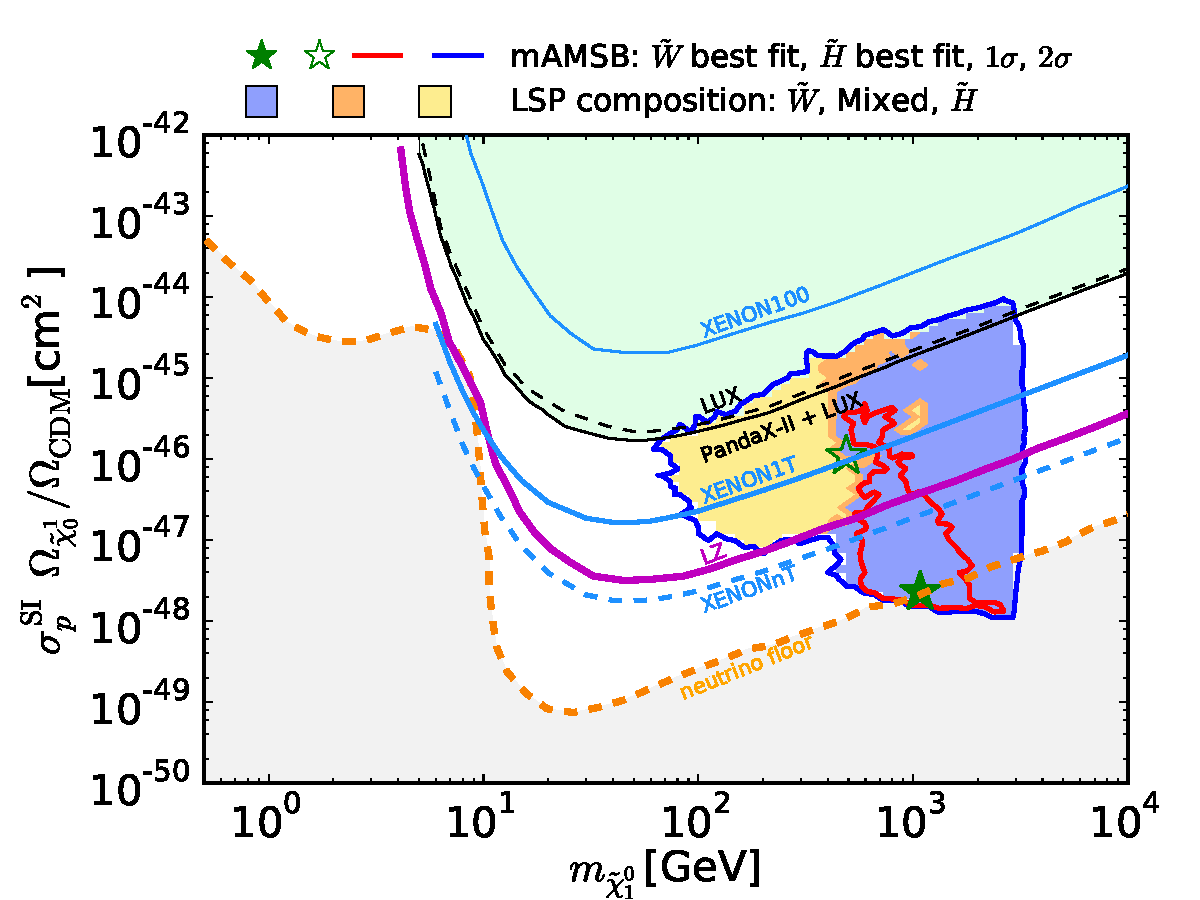
\includegraphics{figs/posmu_noDM_logabsmneu1_SNOW_logssikocm2_SNOW_oh2scaled_chi2.pdf}}\put(-95, +123){\footnotesize $\mu>0$, $\Omega_{\tilde{\chi}_1^0}<\Omega_{\rm CDM}$}%top right
\resizebox{7.5cm}{!}{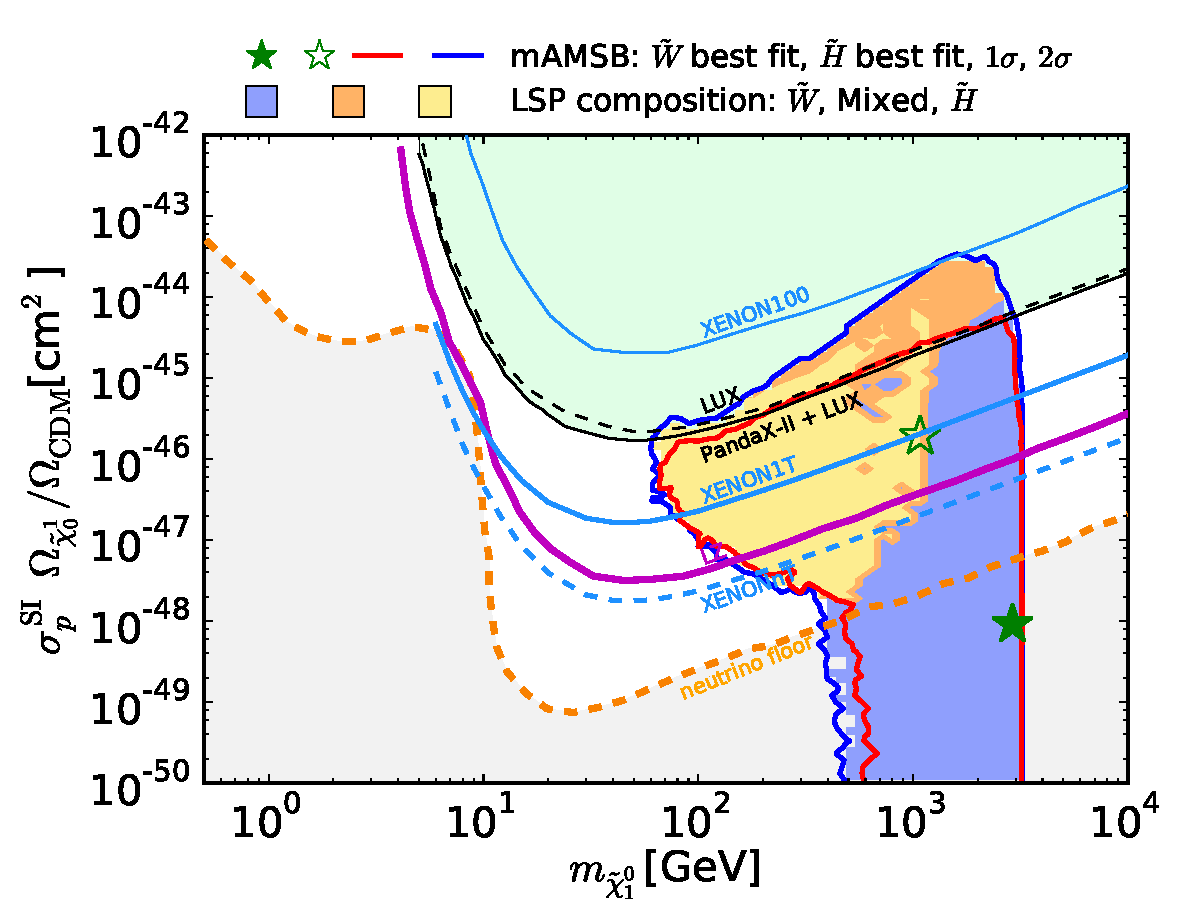
\includegraphics{figs/negmu_noDM_logabsmneu1_SNOW_logssikocm2_SNOW_oh2scaled_chi2.pdf}}\put(-95, +123){\footnotesize $\mu<0$, $\Omega_{\tilde{\chi}_1^0}<\Omega_{\rm CDM}$}%top right
\end{center}
\caption{The $(m_{\tilde{\chi}_1^0}, \sigma_p^{\rm SI})$ planes in the mAMSB for $\mu>0$ (left)
and $\mu<0$ (right) in the case when the LSP only accounts for a fraction of the CDM density. 
The best-fit points for the two signs of $\mu$ are indicated by green stars, closed in the
wino-like region and open in the Higgsino-like region.}
\label{fig:DMdirect_ul}
\end{figure}
%%% the renormaliztion group equations exhibit a novel "focus point" (as opposed to fixed point) behavior, which allows squark and slepton masses far above theirusual naturarlness bounds
%%% anomaly-mediated SUSY breaking parameters 
%%% the susy breaking parameters are then evolved with one-loop RG equations to the superparticle mass scale, m_SUSY
%%% beta functions in hep-ph/9907319v1
%%% mAMSB: ew symmmetry is broken raditively due to the large top quark mass
%%% GUT scale boundary conditions

\begin{comment}
two neutralino states with defined masses
supergravity?
check consistency in notation
https://arxiv.org/pdf/hep-ph/9907319.pdf
https://arxiv.org/pdf/hep-ph/0006049.pdflllllll
https://arxiv.org/pdf/hep-ph/0101034.pdf
https://arxiv.org/pdf/1004.3297.pdf

%%% UN CONHAZO:
https://arxiv.org/pdf/hep-th/9810155.pdf %%% the very worst
https://arxiv.org/pdf/hep-ph/9904378.pdf
https://arxiv.org/pdf/hep-ph/9909376.pdf
\end{comment}


\subsection{Renormalization Group equations}
\label{sec:renormalization}
%%%% arXiv:hep-ph/9709356v7

%%Objetivo 
The renormalization grop equations(RGE) are applied within the MSSM to describe the evolution of gauge couplings, superpotential parameters and soft terms from a given \textit{input} scale up to near the \textit{electroweak} scale. The method used in the SM (dimensional regularization, DREG) cannot be used within SUSY, as it introduces a spurious violation of this symmetry. The most common method for it is the dimensional reduction, DRED, with modified minimal subtraction ($\rm \overline{DR}$), as opposed to DREG with modified minimal subtraction ($\rm \overline{MS}$). 
%% the boundary conditions at the input scale should presumably be applied in a supersymmetry-preerving scheme like DR
Figure \ref{fig:RGE} compares the RG evolution of the coupling constants both in the SM and in the MSSM. As it can be seen, a better match at the electroweak scale is achieved within the MSSM, as discussed in \ref{sec:introduction}. 

\begin{figure}[htb!]
\begin{center}
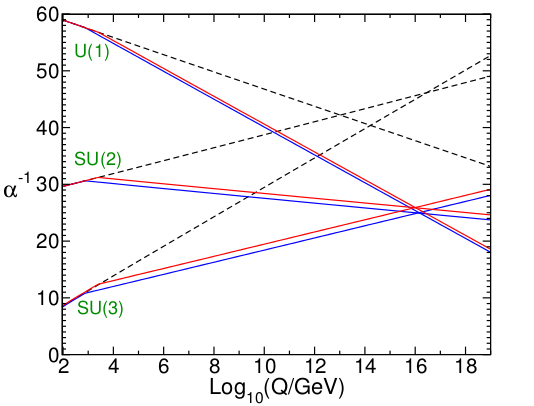
\includegraphics[scale=0.6]{figs/RGE.png}
\end{center}
\caption{Two-loop renormalization group evolution of the inverse gauge couplings $\alpha_a^{-1}(Q)$ in the SM (dashed lines) and the MSSM (solid lines). In the MSSM case, the sparticle masses are treated as a common threshold varied between 750 $\rm GeV$ and 2.5 $\rm TeV$, and $\alpha_3(m_Z)$ is varied between 0.117 and 0.120~\cite{Martin:1997ns}.}
\label{fig:RGE}
\end{figure}

The RGE are derived using what is known as the \textit{supersymmetryc non-renormalization theorem}, that implies that the logarithmically divergent contribution to a particular process can always be written in terms of wave-function renormalizations\red{~\cite{Martin:1997ns}}. One consequence derived from this is that for a given value of $\mu$ \red{at tree-level}, RG corrections to it will be proportional to the parameter itself and some combinations of dimensionless couplings, thus avoiding very large radiative corrections that could greatly enhance $\mu$. 

Within this framework, it is asumed that gauge couplings unify at a given scale, $\Lambda$. Hence, gaugino masses are considered to be unified near that scale as well (which come naturally in GUT models):
\begin{equation}
\frac{M_1}{g_1^2} = \frac{M_2}{g_2^2} = \frac{M_3}{g_3^2} = \frac{m_{1/2}}{g_{\Lambda}^2}
\end{equation}

where $g_\Lambda$ is the unified gauge coupling at $\Lambda$, and $m_{1/2}$ the unification value for the gaugino masses.

%%Consecuencias
Some more consequences of the RGE are listed below. 

\begin{enumerate}
\item Because they are not protected by the supersymmetric non-renormalization theorem, the soft parameters that describe the Yukawa couplings don't vanish at the electroweak scale, even if they are zero at the input scale. %%% not protected by the supersymmetryc non-renormalization
\item The scalar squared masses will be almost diagonal, with the second family squarks and sleptons very nearly degenerate. The third-family squarks and sleptons will get normalized differently 
\item The scalar squared-mass parameters grow as they are RG-evolved, due to the gaugino masses effect on the RGE. Therefore, large masses can be obtained at the electroweak scale even if these are small or even zero at the weak scale. 
\item Because of the contributions they receive from the RGE, the Higgs squared masses generally decrease at the electroweak scale with respect to the input scale. This can lead to a negative value of $m_{H_u}^2$, with the consequence of a non-zero Higgs vev. This effect increases as the top Yukawa coupling does. %%% Thus a large top Yukawa coupling favors the breakdown of the electroweak symmetry breaking because it induces negative radiative corrections to the Higgs squared mass. These facts make it plausible that the Higgs scalars in the MSSM get VEVs, while the squarks and sleptons, having large positive squared mass, do not.
\item If the gaugino mass parameters $M_1$, $M_2$ and $M_3$ have non-zero values for a given input scale, all the soft terms will be generated via RGE. Otherwise, gauginos would be extremely light, causing the model to be inviable due to experimental measurements.%%This implies that models in which gaugino masses dominate over all other effects in the soft supersymmetry breaking Lagrangian at the input scale can be viable.
\end{enumerate}

\section{RPV Models}
\label{sec:RPV}
%%% arXiv:hep-ph/9709356v7
%%% arXiv:1401.7989v4
%%% 
R-parity (or matter parity) conservation can be justified in terms of a grand unified theory or as a consequence of a residual symmetry of a superstring vacuum. However, it is not necessarily the existing scenario. Additional terms can be added to the superpotential in \ref{eq:superpotential} that violate baryon number (B) or lepton number (L), namely: \red{check consistency with other equation}
\begin{equation}
W_{\Delta L=1} = \frac{1}{2}\lambda^{ijk}L_iL_j\overline{e}_k + \lambda'^{ijk}L_iQ_j\overline{d}_k + \mu'^i L_i H_u 
\label{eq:DL}
\end{equation}
\begin{equation}
W_{\Delta B=1} = \frac{1}{2}\lambda''^{ijk}\overline{u}_i\overline{d}_j\overline{d}_k
\label{eq:DB}
\end{equation}
Where $i=1,2,3$, depending on the fermionic family. Terms in \ref{eq:DL} (\ref{eq:BL}) violate lepton (baryon) number by 1 unit. If both terms accompanying $\lambda'$ and $\lambda''$ were to exist (without suppression), proton decays to final products such as $e^+\pi^0$ would be feasible. Nevertheless, the lifetime for the proton is known to be $> 10^{34}$ years\red{~\cite{Nishino:2009aa}}. This, together with more experimental evidence , leads to the conclusion that one of these couplings must be zero or very small, being RPV models either B-violating or L-violating, with experimental upper bounds existing for both couplings. 

One example of such type of RPV model is a scenario where R-parity is replaced by a \textit{baryon triality}, defined in \ref{eq:triality}.
\begin{equation}
Z_3^B = \exp{2\pi i[B-2Y]/3}
\label{eq:triality}
\end{equation}
The corresponding symmetry establishes that the product of the baryon trialities of the particles in any term in the superpotential must be 1. With this, proton decay and neutron-antineutron oscillation are forbidden processes, as they would violate triality. This symmetry does allow the LSP to decay. 

Another alternative is the spontaneous R-parity symmetry breaking by particles, like sneutrinos in the context of MSSM(~\cite{MASIERO1990273},~\cite{ROMAO1992311}). Strong experimental bounds exist on this\red{ref?}. Either way, RPV scenarios greatly change the SUSY signatures in colliders, allowing processes like single sfermion production or exchange of sfermions to happen. %% \red{ref,A. Masiero and J.W.F. Valle, Phys. Lett. B 251, 273 (1990); J.C. Romao, C.A. Santos and J.W.F. Valle, Phys. Lett. B 288, 311 (1992)}

\subsection{Consequences of RPV}
\label{sec:RPVcons}
Numerous consequences can be derived in the different possible RPV models. Some of them are briefly addressed below. 
\begin{enumerate}
\item Within some of these models, there can be \textit{leptogenesis} (asymmetry between leptons and antileptons in the early Universe), that would lead to the current matter-antimatter asymmetry discussed in \ref{sec:introduction}.
\item The LSP can have color/charge, while fulfilling current constraints, and no longer needs to be stable. 
\item Some RPV models include a seesaw mechanism that provides neutrinos with mass, while including sterile neutrinos~\cite{Ghosh:2010hy}.
\item A possible candidate for DM is the heavy gravitino, superpartner of the graviton. Even though it is unstable, its decay is heavily suppressed by the gravitational coupling, resulting in a lifetime bigger than the age of the Universe. 
\end{enumerate}

%%\red{numbers for RP for gauge bosons and gauginos, N=1 SUSY}
%%%% description (marron)
%%%% advantages and disadvantages (red)
%%%% examples (blue)
%%%% experimental signatures (atlas status) 

\section{Experimental searches}
\label{SUSY:exp}

Many experimental efforts have been done in the search for supersymmetry, both via direct searches of supersymmetric particles and by looking for indirect effects. A summary of the former is represented in figures \ref{fig:ATLASSUSYexp} and \ref{fig:CMSSUSYexp}, where bounds on the masses are set for different models, with data from ATLAS and CMS experiments, described in chapter \ref{chap:LHCb}.  

With these experimental constraints, together with other experimental measurements, such as DM direct detection results \ref{} global fits can be made for different SUSY models. A specific case will be discussed in chapter \ref{chap:CMSSM}. More of these fits can be found in~\cite{Athron:2018vxy},~\cite{Athron:2017yua},~\cite{Athron:2017qdc},~\cite{Bagnaschi:2016afc},  
~\cite{Bagnaschi:2016xfg},~\cite{Bagnaschi:2017tru},~\cite{Costa:2017gup}.

\begin{figure} [htb!]
\begin{center}
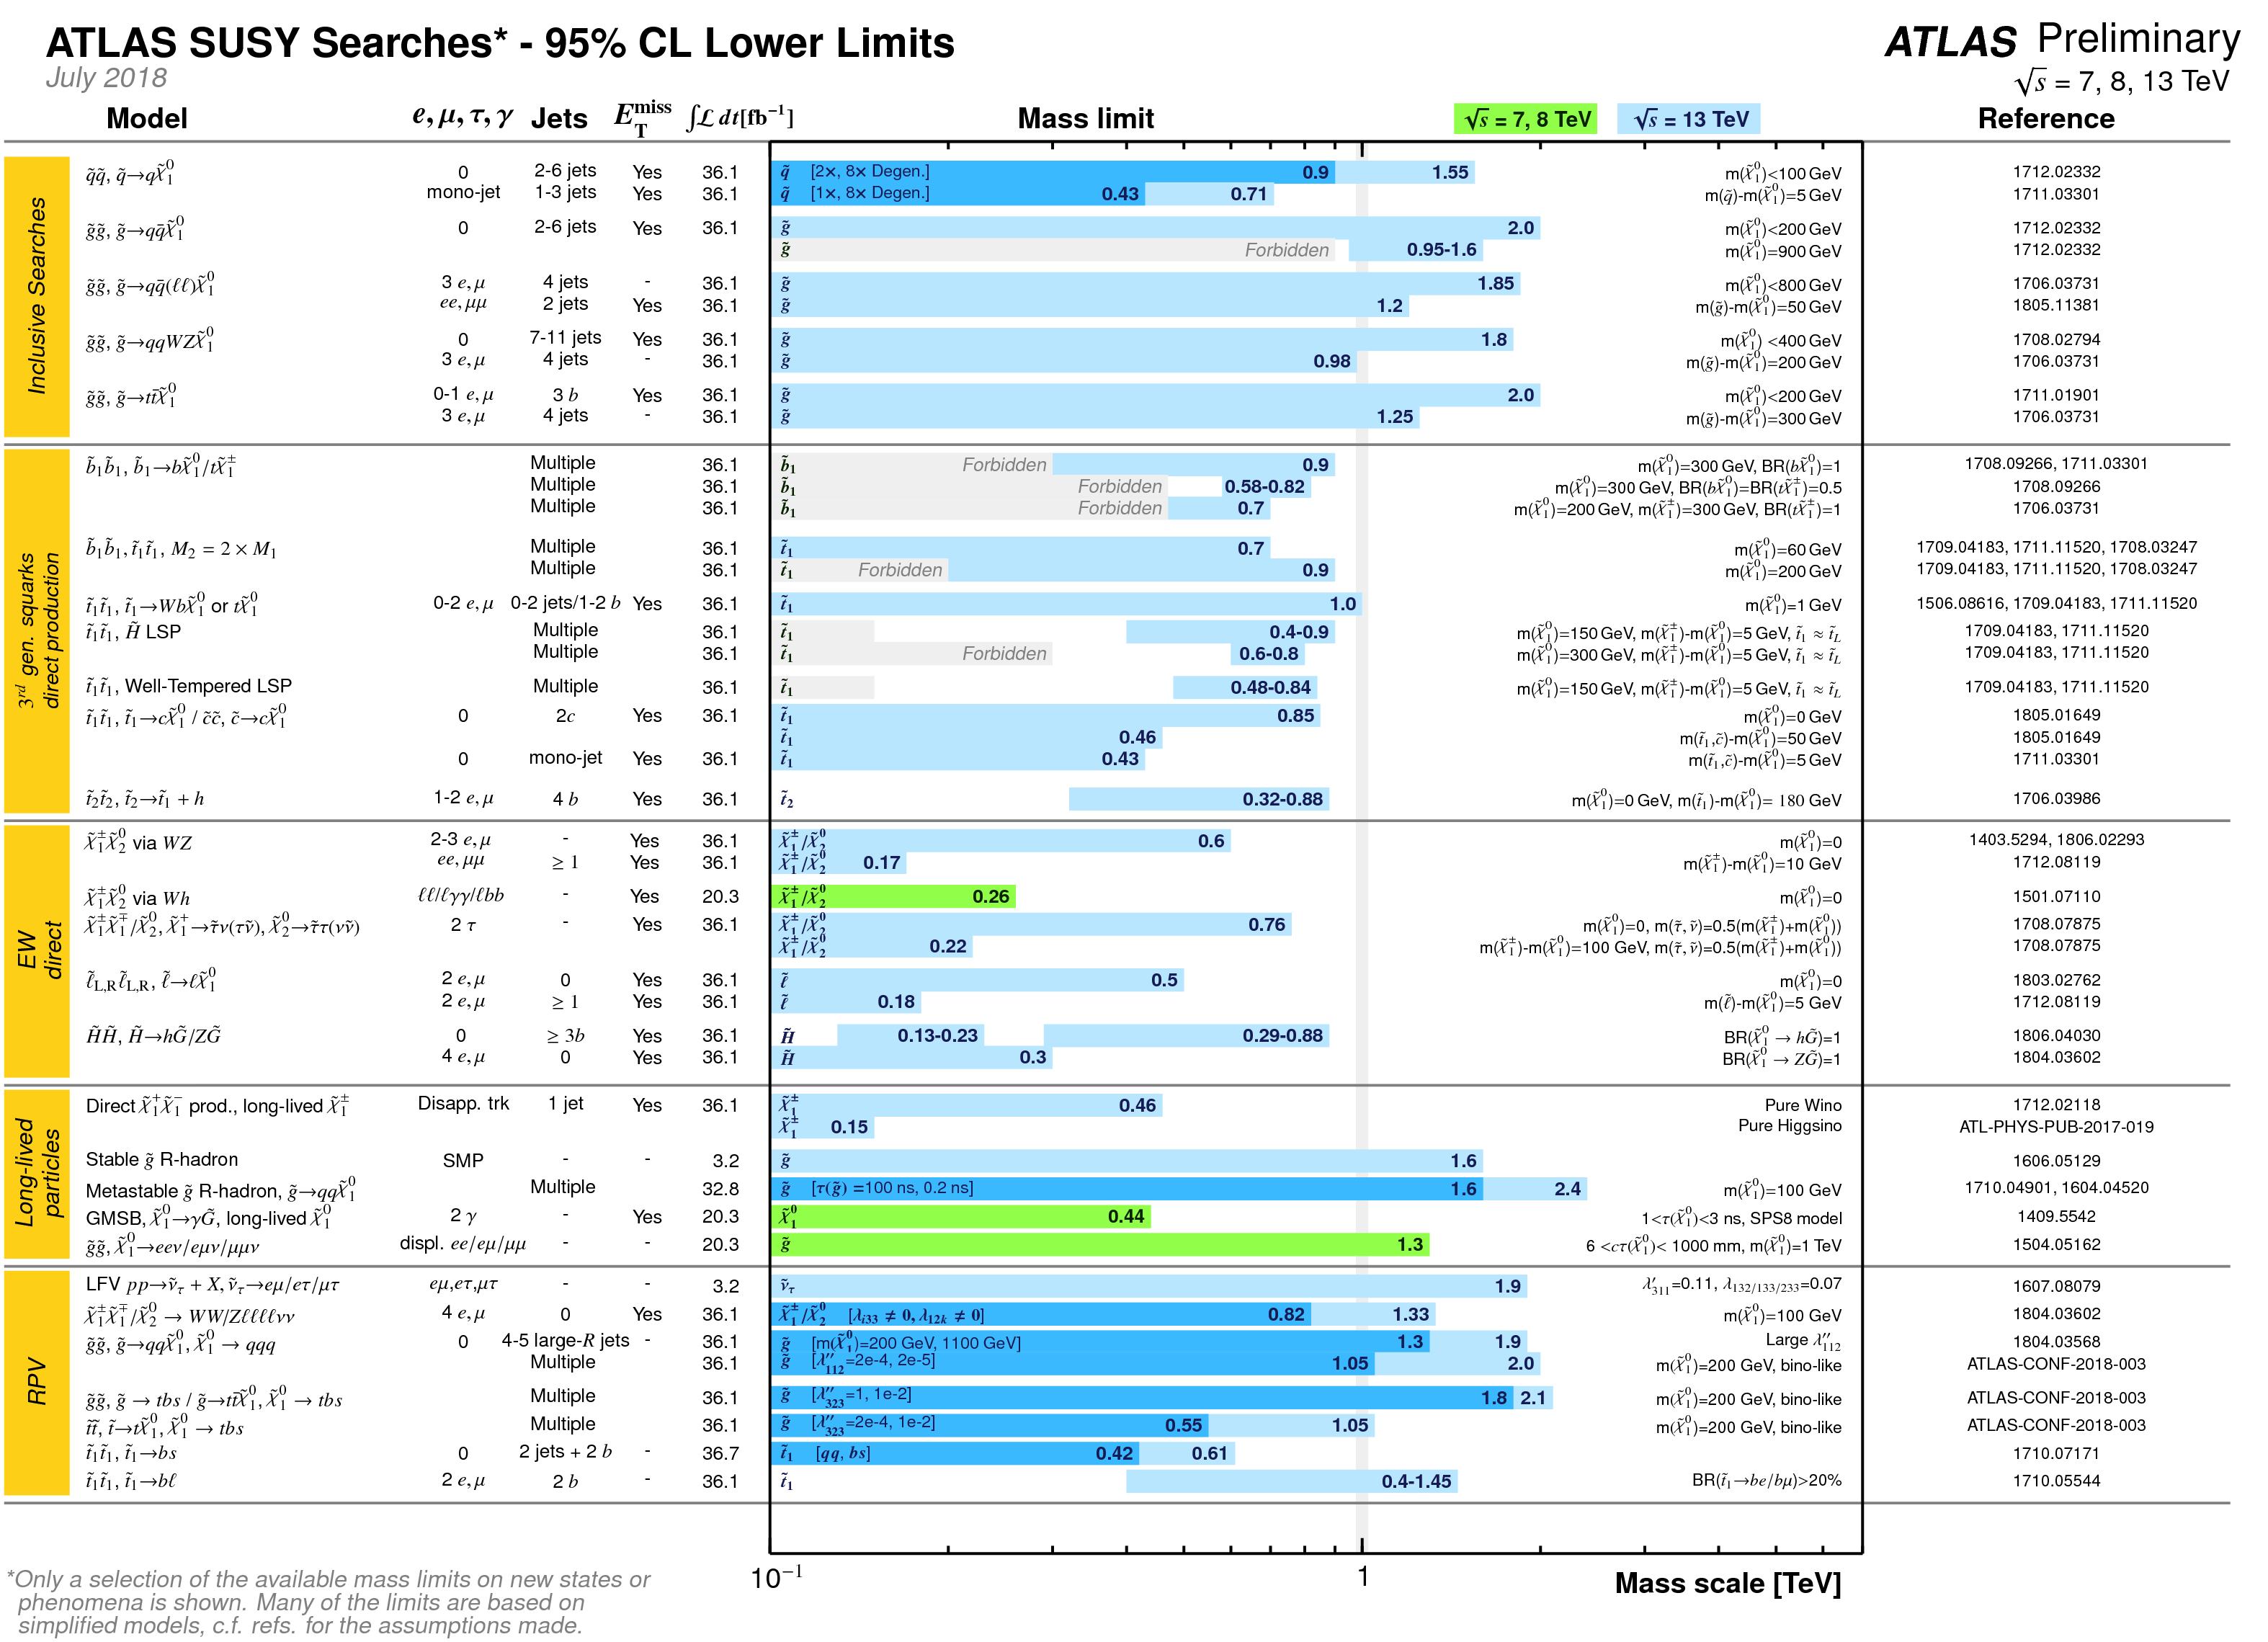
\includegraphics[scale=0.15]{figs/ATLAS_SUSY_Summary.png}
\caption{Experimental status of SUSY searches in ATLAS\label{fig:ATLASSUSYexp} \red{ref}}
\end{center}
\end{figure}

\begin{figure} [htb!]
\begin{center}
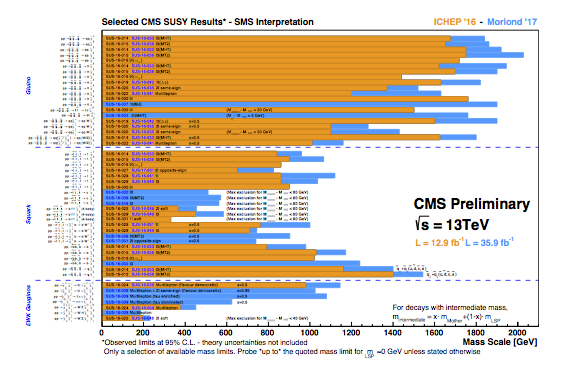
\includegraphics[scale=0.70]{figs/CMS_SUSY_Summary.png}
\caption{Experimental status of SUSY searches at CMS\label{fig:CMSSUSYexp} \red{ref}}
\end{center}
\end{figure}


